% Fig. 1 candidate: the full pipeline, two-column width (7.16 in = 516 pt).
% Build: pdflatex system_overview.tex
\documentclass[tikz,border=1pt]{standalone}
\usepackage[T1]{fontenc}
\usepackage{newtxtext,newtxmath}
\usetikzlibrary{positioning,arrows.meta,fit,backgrounds,calc}

\definecolor{ours}{HTML}{2A78D6}
\definecolor{oursbg}{HTML}{E8F1FC}
\definecolor{learn}{HTML}{0F8A5F}
\definecolor{alarm}{HTML}{D03B3B}
\definecolor{ink}{HTML}{0B0B0B}
\definecolor{muted}{HTML}{52514E}
\definecolor{rule}{HTML}{BDBCB6}

\tikzset{
  font=\footnotesize,
  >={Stealth[length=3.6pt,width=3pt]},
  flow/.style={->, line width=0.6pt, draw=ink},
  box/.style={draw=ink, line width=0.55pt, rounded corners=2pt, align=center,
              minimum height=10.5mm, inner sep=2pt, fill=white},
  snn/.style={box, draw=ours, fill=oursbg},
  data/.style={font=\scriptsize\itshape, text=muted, align=center, inner sep=1.2pt},
  group/.style={draw=rule, dashed, line width=0.45pt, rounded corners=3pt,
                inner xsep=3.5pt, inner ysep=4pt},
  tag/.style={font=\scriptsize\bfseries, text=muted, anchor=south west, inner sep=1.5pt},
  note/.style={font=\scriptsize\itshape, text=muted, anchor=north, inner sep=1.5pt},
}

\begin{document}
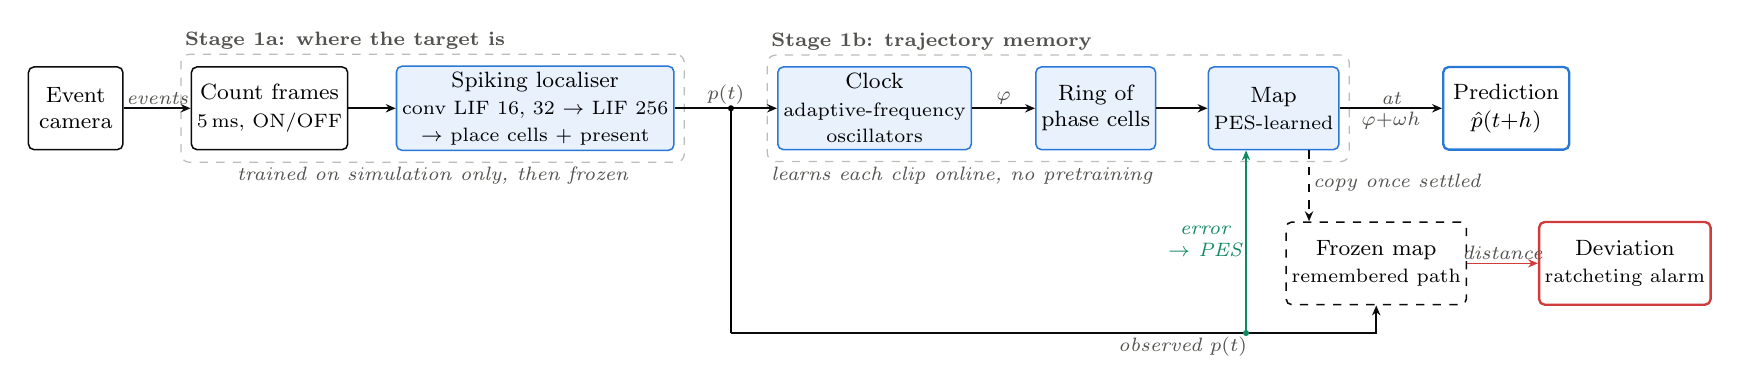
\begin{tikzpicture}[node distance=4mm and 6.5mm]

% --- top row --------------------------------------------------------------------------
\node[box, minimum width=12mm] (cam) {Event\\camera};
\node[box, right=8.5mm of cam, minimum width=19mm] (frames) {Count frames\\[0.5pt]{\scriptsize 5\,ms, ON/OFF}};
\node[snn, right=6mm of frames, minimum width=27mm] (loc)
  {Spiking localiser\\[0.5pt]{\scriptsize conv LIF 16, 32 $\to$ LIF 256}\\{\scriptsize $\to$ place cells + present}};
\node[snn, right=13mm of loc, minimum width=20mm] (clock)
  {Clock\\[0.5pt]{\scriptsize adaptive-frequency}\\{\scriptsize oscillators}};
\node[snn, right=8mm of clock, minimum width=15mm] (ring) {Ring of\\phase cells};
\node[snn, right=6.5mm of ring, minimum width=15mm] (map) {Map\\[0.5pt]{\scriptsize PES-learned}};
\node[box, right=13mm of map, minimum width=16mm, draw=ours, line width=0.85pt] (pred)
  {Prediction\\[0.5pt]$\hat{p}(t{+}h)$};

% --- bottom row: frozen copy and alarm --------------------------------------------------
\node[box, dashed, minimum width=16mm, anchor=north west] (snap)
  at ($(map.south) + (1.5mm,-9mm)$) {Frozen map\\[0.5pt]{\scriptsize remembered path}};
\node[box, right=9mm of snap, minimum width=16mm, draw=alarm, line width=0.85pt] (alarm)
  {Deviation\\[0.5pt]{\scriptsize ratcheting alarm}};

% --- main flow --------------------------------------------------------------------------
\draw[flow] (cam) -- node[data, above] {events} (frames);
\draw[flow] (frames) -- (loc);
\draw[flow] (loc) -- node[data, above, pos=0.5] {$p(t)$} (clock);
\draw[flow] (clock) -- node[data, above] {$\varphi$} (ring);
\draw[flow] (ring) -- (map);
\draw[flow] (map) -- node[data, above] {at} node[data, below] {$\varphi{+}\omega h$} (pred);

% --- observed position: teaches the map, compared with the frozen copy ---------------------
\coordinate (tap) at ($(loc.east)!0.55!(clock.west)$);
\coordinate (low) at ($(tap |- snap.south) + (0,-3.5mm)$);
\draw[line width=0.6pt] (tap) -- (low);
\fill (tap) circle (1.1pt);
\draw[flow] (low) -| node[data, below, pos=0.35] {observed $p(t)$} (snap.south);
\coordinate (pes) at ($(map.south) + (-3.5mm,0)$);
\fill[learn] (pes |- low) circle (1.1pt);
\draw[flow, draw=learn] (pes |- low) -- node[data, text=learn, left, pos=0.5] {error\\$\to$ PES} (pes);
\coordinate (cp) at ($(map.south) + (4.5mm,0)$);
\draw[flow, dashed] (cp) -- node[data, right, pos=0.45] {copy once settled} (cp |- snap.north);
\draw[flow, draw=alarm] (snap) -- node[data, above] {distance} (alarm);

% --- stage groups -----------------------------------------------------------------------
\begin{scope}[on background layer]
  \node[group, fit=(frames)(loc)] (g1) {};
  \node[group, fit=(clock)(ring)(map)] (g2) {};
\end{scope}
\node[tag] at (g1.north west) {Stage 1a: where the target is};
\node[tag] at (g2.north west) {Stage 1b: trajectory memory};
\node[note] at (g1.south) {trained on simulation only, then frozen};
\node[note, anchor=north west] at (g2.south west) {learns each clip online, no pretraining};

\end{tikzpicture}
\end{document}
